\documentclass[conference]{IEEEtran}
\usepackage{cite}
\usepackage{amsmath}
\usepackage{graphicx}
\usepackage{booktabs}
\usepackage{array}
\usepackage[table]{xcolor}
\usepackage[caption=false,font=footnotesize]{subfig}
\usepackage{url}

\graphicspath{{figures/}}

\newcommand{\todo}[1]{\textcolor{red}{[#1]}}

\begin{document}

\title{A Computational Readability Evaluation for Assessing AI Transcription
Readiness of Physical Documents}

\author{
\IEEEauthorblockN{Lore Lawlor}
\IEEEauthorblockA{\textit{Nick Howley College of Engineering and Computing}\\
Drexel University\\
Philadelphia, PA\\
}
\and
\IEEEauthorblockN{Simm Vallaban}
\IEEEauthorblockA{\textit{College of Engineering}\\
Temple University\\
Philadelphia, PA\\
}
\and
\IEEEauthorblockN{Author Three}
\IEEEauthorblockA{\textit{Department / Organization}\\
City, Country\\
email}
}

\maketitle

\begin{abstract}
The accuracy of optical character recognition (OCR) output depends in part on
the quality and legibility of the original physical document. Preprocessing
improves the quality of scanned images, but it is computationally expensive to
run on every scan in a large collection. Evaluating each document's readability
in advance shows which ones need additional processing before transcription.
This paper presents an approach for assessing the machine readability of
handwritten scientific documents, with a preliminary implementation and
evaluation of a quantitative readability score. The approach uses three
computational metrics to score the baseline consistency, spatial organization,
and text fragmentation of a page from each of the three chosen handwritten
chemistry student lab notebooks from students studying MOFs (Metal Organic
Frameworks). These notebooks are categorized as having neat, average, and messy
handwriting styles and scored on a scale from 0 (low readability) to 1 (high
readability). The resulting score is then compared to transcription accuracy,
measured as character error rate (CER), which is manually determined through
the authors' establishment of a ground truth. The readability score ranked the
pages in the same order as the CER (Pearson $r = -0.882$; Spearman
$\rho = -1.000$). Pages with a higher readability score provided lower
transcription error results. OCR confidence, which is a metric determined by
the OCR which predicts the perceived success of the transcription, by contrast
was positively correlated with CER ($r = 0.674$; $\rho = 0.500$). However, all
scores fell within a narrow range, and error rates were high for every page
(68--77\% CER); therefore, this study should serve as a first test of the
approach. This methodology should help prioritize preprocessing and inform
evidence-based recommendations for documentation practices that support the
machine readability of handwritten scientific documents.
\end{abstract}

\begin{IEEEkeywords}
handwritten documents, optical character recognition, OCR, machine readability, laboratory notebooks, character error rate
\end{IEEEkeywords}

\section{Introduction}
Handwritten lab notebooks are both records of experiments and documentation of
student learning. For this information to be used by researchers and in AI
analysis, it must first be digitized. Converting these lab notebooks or other
handwritten documents into digital transcriptions depends on the application of
optical character recognition (OCR) tools to scanned copies of the lab
notebooks' pages. The accuracy of these tools, however, depends partly on the
quality of the input provided \cite{ye2013, alaei2024}. Preprocessing scans of
handwritten documents can improve input quality and make a document more
machine-readable \cite{sauvola2000, gonzalez2018}, but is an expensive process
in computing time and effort for large collections.
Because there is no simple way to determine which scans may require
preprocessing, assessing each notebook's readability before transcription would
enhance the transcription pipeline's efficiency.

The notebooks used in this study originate from the Reticular Synthesis and
Materials Design Lab (RSMDL) of Dr.\ Fernando Uribe-Romo of the University of
Central Florida's Chemistry Department, which studies metal organic frameworks
(MOFs). The effort to digitize these notebooks is a part of the NSF-HDR
Institute for Data-Driven Dynamical Design in conjunction with the Metadata
Research Center at Drexel University. Earlier work using MOF students' lab
notebooks returned table-cell error rates of 4\% to 18\%, depending on the OCR
tool used for transcription and the correction steps taken \cite{pepper2025},
and these results support checking scan quality before transcription.

This paper presents a preliminary approach to assessing handwritten scientific
documents for machine readability before OCR transcription. The section that
follows provides a brief background on the use of analog notebooks in labs,
defines Computational Archival Science (CAS), and details how it relates to our
research. Next, we state our research goals and describe the methods used to
compute a readability score and compare it with transcription error. Finally,
we discuss results and future work, identify next steps, and present our
conclusions.

\section{Background: Analog Laboratory Notebooks and CAS}
Low barrier to adoption and use, reasonable cost, and portability are the
principal reasons why scientists use physical lab notebooks in wet labs instead
of electronic ones \cite{kanza2017}. In addition to these advantages,
handwritten historical documents and modern physical records do not depend on
software and can outlast rapidly evolving technology \cite{ryan2007}. However,
to be shared, reproduced, and analyzed, physical lab notebooks and other
handwritten documents must be digitally transcribed. Transcription at scale
requires a reliable transcription pipeline so that the data remains accurate,
and the processing time reasonable.

Computational Archival Science (CAS) addresses the need for the efficient and
reliable processing of records by combining archival science, computer science,
and subject expertise to develop scalable and automated methods for management
\cite{marciano2018}. A lab notebook can be defined as an archival record since
it documents the steps, observations, and results of an experiment. This
observation draws from foundational archival theory which holds that a record's
meaning depends on its provenance, the context in which it was created and its
original order, the sequence or positioning in how it was kept
\cite{jenkinson1922}. CAS principles call for archival records such as these to
remain reliable and authentic, as well as connected to their original context
when converted to digital form \cite{hedges2022}. Our proposed readability
score aims to support reliability by identifying which scans require further
processing. This allows the visual quality of the scans to be improved before
transcription, which makes the output more accurate and keeps the transcription
pipeline efficient.

\section{Goals and Objectives}
An overall motivating goal of our research is to create a method in which
physical lab notebooks may be reliably transcribed and ultimately added to a
database which can be queried with pedagogical inquiries and mined for
additional information and insights. The immediate goal of the research
presented in this paper is to define an approach for assessing the machine
readability of scanned handwritten lab notebooks using computational methods
before OCR transcription. The goal has three objectives:
\begin{itemize}
  \item Measure baseline consistency, spatial organization, and text
        fragmentation from scanned notebook pages without using an OCR tool.
  \item Combine the resulting measurements into a single readability score on a
        scale of 0 (low readability) to 1 (high readability).
  \item Compare the readability score to the CER of OCR transcriptions from
        notebooks categorized as neat, average, and messy handwriting.
\end{itemize}

\section{Methods}
\label{sec:methods}
To address our goals, this study developed and evaluated a computational method
for quantifying structural characteristics to determine whether the measurable
visual properties of laboratory notebook pages can predict OCR transcription
performance without using the OCR tool itself. The methodology was informed by
research on the variability of handwriting \cite{papavassiliou2010, rabaev2026},
prior work on scientific document recognition \cite{pepper2025}, document image
quality \cite{ye2013, alaei2024}, and OCR evaluation
\cite{smith2007, levenshtein1966}. These areas were fundamental in guiding the
selection of structural features and validation metrics.

\subsection{Data}
\label{sec:data}
One representative page ($1455 \times 1980$ pixels) from each of the three
chosen student lab notebooks was scanned. Then, a MOF researcher visually
assessed the notebook scans and grouped them by handwriting style as neat,
average, or messy, as seen in Fig.~\ref{fig:styles}.

\begin{figure*}[t]
  \centering
  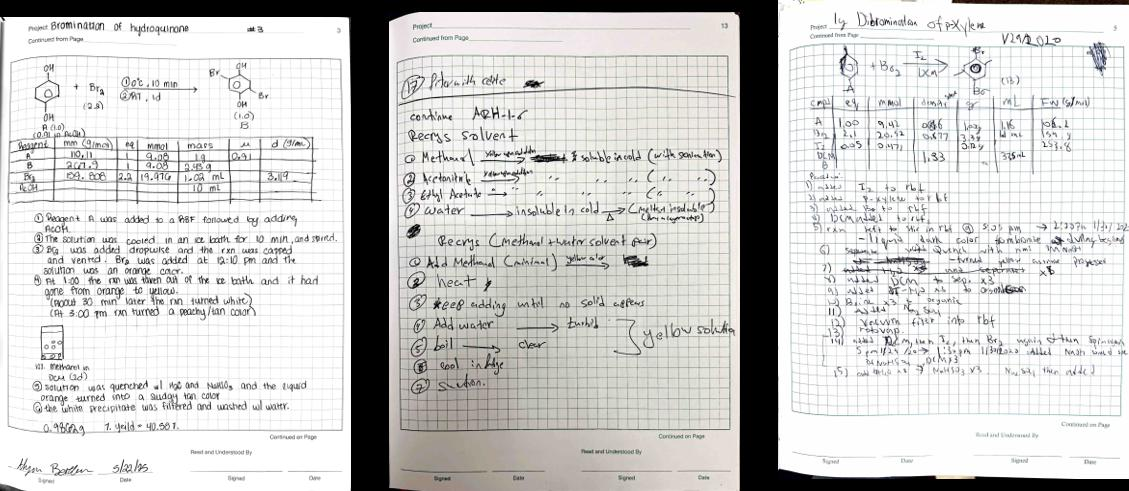
\includegraphics[width=0.85\textwidth]{fig1_handwriting_styles.png}
  \caption{(from left to right) neat, average, and messy handwriting styles
  from students' chemistry lab notebooks from Dr.\ Fernando Uribe-Romo at the
  University of Central Florida.}
  \label{fig:styles}
\end{figure*}

Each page was prepared (Section~\ref{sec:methods}-\ref{sec:prep}) using
grayscale conversion, adaptive thresholding, and morphological opening. Three
structural measurements were taken from the prepared image: baseline
consistency ($b$), spatial organization ($s$), and text fragmentation ($f$).
These were combined into a readability score using a weighted formula,
resulting in a value from 0 (low readability) to 1 (high readability). All
image processing used Python 3.13 and OpenCV \cite{bradski2000}. The readability score was
then compared to the CER of the OCR transcription, which is obtained via manual
review by the authors.

To test whether higher readability could coincide with lower transcription
error, each original, unprepared scan was transcribed with Tesseract OCR \cite{smith2007, tesseract_manual} through the
pytesseract library \cite{pytesseract}, using its default settings (English
model, automatic page segmentation). The ground truth for each page is a
manual transcription typed by the authors, who entered the text of each scan
into a plain UTF-8 text file with the page's line breaks and reading order being preserved;
no OCR output was used to create it. CER was computed with the JiWER library
\cite{jiwer} as the number of character substitutions, deletions, and
insertions \cite{levenshtein1966} needed to turn the OCR output into the
ground truth, divided by the number of ground-truth characters (997, 463, and
845 for the neat, average, and messy pages). Case and punctuation were kept
and no other text normalization was applied.

OCR confidence is the mean of the word-level confidence scores (0 to 100) that
Tesseract reports through \texttt{pytesseract.image\_to\_data}, averaged over
all words on the page and excluding the $-1$ values Tesseract assigns to
non-word layout entries. Lastly, OCR confidence was compared with both the readability
score and the CER. 

\subsection{Image Preparation}
\label{sec:prep}
OCR tool transcription accuracy depends, in part, on how effectively the system
can distinguish between handwritten text and the surrounding document image.
Inconsistencies such as background shadows, uneven illumination of the scanned
document page, page texture, and isolated image noise can be mistaken for
handwriting and hinder the proper detection of actual handwritten characters
\cite{smith2007}. For example, a faint decimal point can be lost during
thresholding, while disconnected strokes can cause a single character to be
represented as multiple different components in the image \cite{fujisawa1992}.
Similarly, adjacent characters can merge into one foreground region, thus
making segmentation more difficult. Errors such as these can propagate through
the OCR transcription pipeline and can raise the error rate of the final
transcription. Document image quality affects both structural feature
extraction and OCR performance following an approach by Alaei \emph{et al.}
\cite{alaei2024}. Image preparation removes this noise so that it does not
distort the final readability score.

\begin{figure}[t]
  \centering
  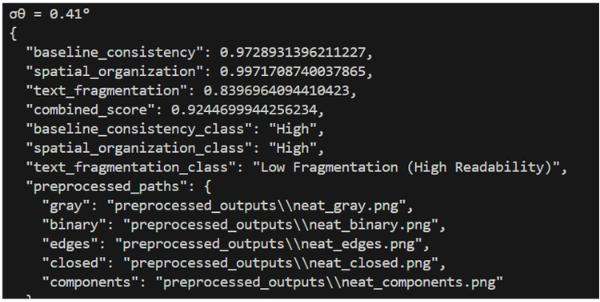
\includegraphics[width=\columnwidth]{fig2_script_output.png}
  \caption{Readability scoring output (Python 3.13) for the neat notebook page:
  baseline angle deviation ($\sigma_\theta$), the three metric scores, the
  combined score, and the class of each metric from Table~\ref{tab:bands}.}
  \label{fig:output}
\end{figure}

The first preparation stage, grayscale conversion, reduces each pixel from
multiple color channels to a single intensity representation, simplifying the
subsequent image analysis when ink color itself is not a variable being
evaluated \cite{gonzalez2018}. Before thresholding, a $3 \times 3$ Gaussian blur is applied to reduce local pixel variation \cite{gonzalez2018, opencv_filtering}. Adaptive thresholding then separates foreground handwriting from the background by computing a separate threshold for each
pixel from a Gaussian-weighted $31 \times 31$ pixel neighborhood with an offset
of 11 gray levels \cite{opencv_misc}. These two settings were chosen by visual inspection of the thresholded output and affect the resulting scores (Section~\ref{sec:discussion}). Unlike global thresholding, which applies one common threshold across the entire image, adaptive thresholding instead responds locally to spatial variations in illumination, which is particularly useful for scans of physical documents \cite{sauvola2000, bradley2007, binmakhashen2019}. The threshold is then inverted so that ink becomes white (foreground) and paper becomes black (background) since OpenCV's morphology
and connected-component functions treat any nonzero (white) pixels as the
object being measured \cite{opencv_morph, opencv_shape}.

Morphological processing provides an additional means of controlling the
geometry and connectivity of foreground regions
\cite{serra1982, haralick1987}. Morphological opening in particular can remove
isolated foreground artifacts through its method of erosion followed by
dilation \cite{haralick1987, gonzalez2018}. This process reduces the likelihood
that image noise will be interpreted as handwriting later in the analysis.
Conversely, morphological closing, which is the reverse of opening in that
dilation is followed by erosion, can reconnect nearby foreground structures and
is used separately when examining text fragmentation
\cite{haralick1987, gonzalez2018}. Closing ($5 \times 5$ kernel, two passes) is
applied only when measuring text fragmentation (Section~\ref{sec:measure}).


\begin{figure*}[t]
  \centering
  \subfloat[]{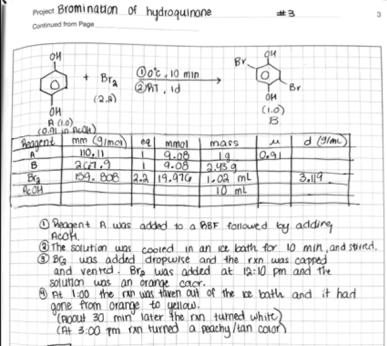
\includegraphics[width=0.19\textwidth]{fig3a_grayscale.png}}\hfill
  \subfloat[]{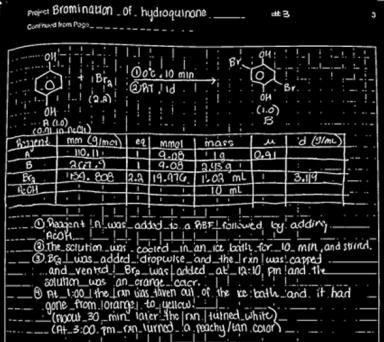
\includegraphics[width=0.19\textwidth]{fig3b_threshold_opening.png}}\hfill
  \subfloat[]{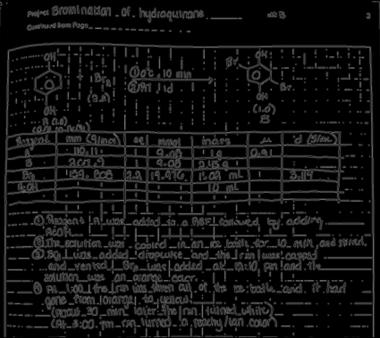
\includegraphics[width=0.19\textwidth]{fig3c_canny_edges.png}}\hfill
  \subfloat[]{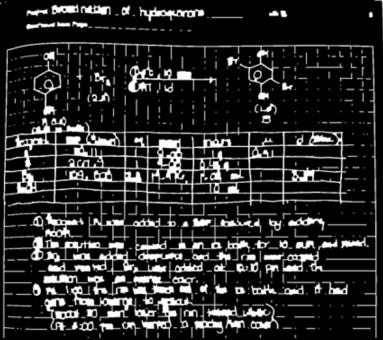
\includegraphics[width=0.19\textwidth]{fig3d_closing.png}}\hfill
  \subfloat[]{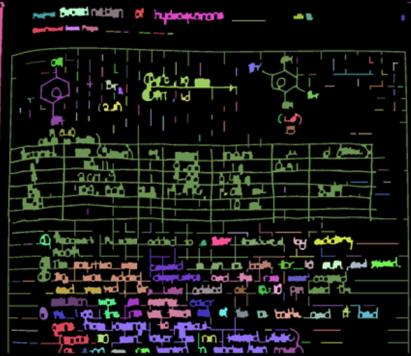
\includegraphics[width=0.19\textwidth]{fig3e_components.png}}
  \caption{Image preparation for the neat notebook page, in processing order.
  (a) Grayscale conversion of the original scan.
  (b) Adaptive thresholding (inverted) followed by morphological opening; ink is
  white because OpenCV measures nonzero pixels as foreground.
  (c) Canny edge map of (b) \cite{canny1986}, shown for illustration only;
  no metric uses it.
  (d) Morphological closing of (b), which joins nearby strokes before text
  fragmentation is measured.
  (e) Connected components of (d), each shown in a different color.}
  \label{fig:prep}
\end{figure*}

\subsection{Readability Measurements}
\label{sec:measure}

Handwritten documents inherently exhibit variation in defining characteristics
like baseline fluctuations, irregular inter-line spacing, variable character
dimensions and overlapping characters, which complicate text-line segmentation
and recognition \cite{papavassiliou2010, rabaev2026}. Following image
preparation, three structural metrics are identified: baseline consistency
($b$), spatial organization ($s$), and text fragmentation ($f$). Each was
scaled from 0 to 1 against a reference value, where higher values mean higher
readability.

A reference value is the number each raw measurement is compared against to
place it on the 0 to 1 scale; it marks the point at which the score reaches 0
(or, for the fragmentation terms, the point at which a term reaches its
maximum), and results outside 0 to 1 are clipped. The reference values were
chosen by judgement rather than derived from data or prior work, and are listed
for each metric below and in Table~\ref{tab:reference}.
The structural metrics evaluated, including their associated analysis, are as
follows:

\begin{itemize}
  \item \textbf{Baseline Consistency ($b$)}
  \begin{itemize}
    \item Measured baseline Angular Variance ($\sigma_\theta$), connected
    component variance, least-squares baseline estimation
    \cite{ogorman1993, opencv_shape}, and a horizontal projection profile
    (count of ink pixels in each row) \cite{likforman2007, papavassiliou2010}
    to determine the standard deviation between baseline angles (low variance
    indicates consistent writing alignment).
    % ADDED (comments [9]-[11]):
    \item Reference value: $15^\circ$. The score is
    $b = 1 - \sigma_\theta / 15^\circ$, so a page whose baseline angles vary by
    $15^\circ$ or more scores 0.
  \end{itemize}

  \item \textbf{Spatial Organization ($s$)}
  \begin{itemize}
    \item Variance of the vertical spacing between band centroids measured via
    horizontal projection profiles computed from a binarized image was used as
    a measure of spatial organization \cite{likforman2007}. This measures how
    consistently text bands are spaced where low-spacing variance means better
    organization and reduced OCR segmentation errors.

    \item Reference value: $H^2/16$, where $H$ is the page height in pixels.
    The score is $s = 1 - \mathrm{Var}(d) / (H^2/16)$, where $\mathrm{Var}(d)$
    is the spacing variance; the reference corresponds to a spacing standard
    deviation of one quarter of the page height (495 pixels for these pages).
  \end{itemize}

  \item \textbf{Text Fragmentation ($f$)}
  \begin{itemize}
    \item Measurements of component density (weighted by judgement at 45\% and
    measures how densely handwriting occupies the page) \cite{fujisawa1992},
    nearest neighbor distance (weighted by judgement at 35\% and measures how
    closely related text regions are where larger distances suggest more
    scattered information) \cite{ogorman1993, clark1954}, and the small
    component ratio (weighted by judgement at 20\% which measures the
    proportion of very small connected components such as broken strokes,
    isolated punctuation, and overall document noise)
    \cite{fujisawa1992, ye2013}, are combined utilizing heuristically-weighted
    coefficients to create composite text fragmentation measurement.
    \item The resulting formula is
    $\text{Fragmentation} = 0.45 \cdot \text{density} + 0.35 \cdot
    \text{nearest neighbor distance} + 0.20 \cdot \text{small\_ratio}$,
    and $f = 1 - \text{Fragmentation}$. This resulting fragmentation value is
    presented on a 0 to 1 scale, where a higher $f$ means lower fragmentation
    and high readability.
  \end{itemize}
\end{itemize}

\begin{table}[!t]
  \centering
  \caption{Reference values used to scale each raw measurement to 0--1. All
  were chosen by judgement.}
  \label{tab:reference}
  \footnotesize
  \setlength{\tabcolsep}{3pt}
  \renewcommand{\arraystretch}{1.15}
  \begin{tabular}{@{}>{\raggedright\arraybackslash}p{2.1cm}>{\raggedright\arraybackslash}p{2.9cm}>{\raggedright\arraybackslash}p{3.3cm}@{}}
    \toprule
    Metric or term & Raw measurement & Reference value \\
    \midrule
    $b$ & Standard deviation of baseline angles, $\sigma_\theta$ & $15^\circ$ ($b = 0$ at or above) \\
    $s$ & Variance of band spacing & $H^2/16$ (standard deviation of 495 px) \\
    $f$: component density & Components per ink pixel & $\times 40$, capped at 1 \\
    $f$: nearest neighbor distance & Mean distance to nearest component & Square root of page area (1697 px) \\
    $f$: small component ratio & Share of components under 150 px & None (already a proportion) \\
    \bottomrule
  \end{tabular}
\end{table}

\subsection{Combined Readability Score}
The combined score is then calculated using a heuristically weighted average
$0.40b + 0.20s + 0.40f$, resulting in a 0--1 score.

Baseline consistency and text fragmentation were weighted more heavily than
spatial organization because we judged line alignment and broken or merged
strokes to affect OCR more directly than the spacing between lines; no prior
work supplies weights for these metrics.
Depending on the final determined score, each metric and the overall
readability may be indicated as either `High', `Moderate', or `Low', as shown
in Table~\ref{tab:bands}.

The cut-offs at 0.80 and 0.50 were chosen by judgement and apply to each metric and to the combined score. Finally, a statistical evaluation is performed to compare the readability score against manually calculated CER (character error rate), and OCR confidence
rate.

\begin{table}[!t]
  \centering
  \caption{The final combined score using the weighted formula of
  $0.40b + 0.20s + 0.40f$ results in a 0--1 score. For each metric and the
  combined score, High is defined as 0.80 and above, Moderate 0.50 to 0.79, and
  Low below 0.50.}
  \label{tab:bands}
  \footnotesize
  \setlength{\tabcolsep}{3pt}
  \renewcommand{\arraystretch}{1.15}
  \begin{tabular}{@{}l>{\raggedright\arraybackslash}p{1.45cm}>{\raggedright\arraybackslash}p{1.55cm}>{\raggedright\arraybackslash}p{2.6cm}@{}}
    \toprule
    Score & Baseline Consistency & Spatial Organization & Text Fragmentation \\
    \midrule
    \rowcolor{green!15}
    0.80--1.00 & High     & High     & Low Fragmentation (\emph{High Readability}) \\
    \rowcolor{yellow!20}
    0.50--0.79 & Moderate & Moderate & Moderate Fragmentation \\
    \rowcolor{red!12}
    0.00--0.49 & Low      & Low      & High Fragmentation (\emph{Low Readability}) \\
    \bottomrule
  \end{tabular}
\end{table}

\subsection{Results}
As a way to preliminarily review the effectiveness of the methods above, results are based on one page each of three chosen student lab notebooks.
Combined readability scores all scaled within the high readability range,
measuring between 0.920 and 0.924 (Table~\ref{tab:raw}). Pearson and Spearman
correlations between the readability score and the CER showed a negative
relationship (Pearson $r = -0.882$ and Spearman $\rho = -1.000$), with the pages
being ranked by score in the same order as by the CER.

\begin{table}[t]
  \centering
  \caption{Readability metrics, CER, and OCR confidence for each page.}
  \label{tab:raw}
  \footnotesize
  \setlength{\tabcolsep}{4pt}
  \begin{tabular}{@{}lcccccc@{}}
    \toprule
    Page & $b$ & $s$ & $f$ & Combined & CER & OCR Conf. \\
    \midrule
    Neat    & 0.9729 & 0.9972 & 0.8397 & 0.9245 & 67.7\% & 54.6 \\
    Average & 0.9728 & 0.9975 & 0.8350 & 0.9226 & 75.6\% & 79.9 \\
    Messy   & 0.9406 & 0.9977 & 0.8599 & 0.9197 & 77.2\% & 63.9 \\
    \bottomrule
  \end{tabular}
\end{table}

\begin{table}[t]
  \centering
  \caption{Relationship between readability score, OCR confidence, and CER.}
  \label{tab:corr}
  \footnotesize
  \begin{tabular}{@{}lcc@{}}
    \toprule
    Comparison & Pearson ($r$) & Spearman ($\rho$) \\
    \midrule
    Combined Score vs.\ OCR Confidence & $-0.247$ & $-0.500$ \\
    Combined Score vs.\ CER            & $-0.882$ & $-1.000$ \\
    OCR Confidence vs.\ CER            & $0.674$  & $0.500$  \\
    \bottomrule
  \end{tabular}
\end{table}

OCR confidence was found to have a positive correlation with CER
($r = 0.674$; $\rho = 0.500$), while the correlation between readability score
and OCR confidence was $r = -0.247$ and $\rho = -0.500$
(Table~\ref{tab:corr}).

Baseline consistency remained high for all lab notebook pages that were
evaluated, and exhibited the largest variation in score across all samples
evaluated (0.941 to 0.973). Despite this, with three pages as the sample size,
none of the correlations were statistically significant.

%%%%%%%%%%%%%%%%%%%

\section{Discussion}
\label{sec:discussion}
With this research, we have started to address our goal of assessing machine
readability of handwritten lab notebooks prior to transcription. The
readability score derived from a set of computational methods, independent of
the OCR tool itself, ranked the scanned pages in the same order as the CER and
visual assessment had (Table~\ref{tab:raw}). 

While the readability score ranked the pages accurately compared to the CER,
every page was rated 'High' readability, despite CERs ranging from 68\% to 77\%.
This was our biggest surprise, as identifying scanned images which may be
unreadable to machines is our main use case. Spatial organization ($s$)
provided results with little to no change across the three pages (0.997 to
0.998), which suggests that this metric could be either less consequential to
machine readability, or that the reference value used should be reassessed
during future research.

The reference value for $s$ corresponds to a spacing standard deviation of 495
pixels, about twenty times larger than the spacing variation measured on these
pages (24 to 26 pixels), so nearly any page scores close to 1.
Text fragmentation ($f$) rated the notebook categorized as messy as least
fragmented, which seems contradictory to the visual nature of messy
handwriting. We also found that baseline consistency ($b$) was the most
visually aligned factor for this set, with the messy notebook ranking low in
consistency.

It is also surprising to find that OCR confidence scores can be overstated by
the tool itself. Our results found that the page which was judged by researchers as
'neat' handwriting had the lowest confidence but conversely, the lowest error.
Additionally, the average handwriting page was ranked as the highest
confidence, but had the second highest error (75.6\%). This suggests that
OCR-determined confidence scores alone may not reliably predict or reflect
transcription accuracy, and should be assessed carefully when being used to
predict the truth of document readability.

With three pages, however, this is an observation rather than a finding.

This study has three limitations: small sample size, judgement-based weighting,
and the use of one OCR tool. First, we tested the methods to obtain a
readability score on three pages, one from each notebook; because a sample this
size cannot establish significant results, this study should be seen as an
early attempt at the approach. Second, the weights and values were based on
heuristic scaling; human judgement was used to determine which metrics should
receive higher weight in the readability evaluation. Lastly, the transcription
software Tesseract produced high error rates in transcription. Even for the
notebook pages determined to be neat, both by our visual judgement and by the
combined readability score, error rates were high. This finding suggests that
future work may benefit from the use of multiple transcription tools for
comparison.


%%%%%%%%%%%%%%%%%%%

\section{Conclusion}
In this paper, we propose an approach for assessing the machine readability of
scanned handwritten lab notebooks prior to OCR transcription. This approach
utilizes image processing to quantify baseline consistency, spatial
organization, and text fragmentation. Then, the results are combined into a
score which reports on the document's machine readability without the use of
OCR, which can be expensive or time-consuming to use. In
a preliminary test on three scanned notebook pages, the score ranked the pages
in the same order as their CER, while OCR confidence was found to not
accurately reflect transcription accuracy. The next steps in this research
include expanding our sample size and using multiple OCR tools to compare
results.

Further next steps include testing a wider range of pages, including pages
expected to score low, adjusting the weights and reference values, and
reformulating the text fragmentation metric ($f$).
This work makes progress toward quantifying notebook and handwriting quality, a
step which was identified by our earlier work as sequential to making analog
lab notebooks more AI-ready \cite{pepper2025}. With the development of a
readability check which could reliably report on predicted transcription
accuracy before OCR transcription, notebooks that have never been transcribed
could be selected for transcription pipelines or identified for further
preprocessing prior to their transcription. Digital transcription enables
physical documents to be added to searchable databases where they may be
studied and used by scientists, teachers, and students alike. In time, these
transcriptions may aid in training future tools and inform future physical
documentation practices.

%%%%%%%%%%%%%%%%%%%

\section*{Acknowledgment}
This work was supported by the National Science Foundation through the
Institute for Data-Driven Dynamical Design, OAC-2118201, and the Drexel
University Metadata Research Center. We acknowledge the original authors of the
lab notebooks, Alyssa Bordner, Yuen Lau, and Wesley Newsome, and the
Uribe-Romo lab.


%%%%%%%%%%%%%%%%%%%
\begin{thebibliography}{00}

\bibitem{ye2013}
P. Ye and D. Doermann, ``Document image quality assessment: A brief survey,'' in \emph{Proc. 12th Int. Conf. Document Analysis and Recognition (ICDAR)}, 2013, pp. 723--727. doi: 10.1109/ICDAR.2013.148.

\bibitem{alaei2024}
A. Alaei, V. Bui, D. Doermann, and U. Pal, ``Document image quality assessment: A survey,'' \emph{ACM Computing Surveys}, vol. 56, no. 2, Art. 29, pp. 1--36, 2024. doi: 10.1145/3606692.

\bibitem{sauvola2000}
J. Sauvola and M. Pietik{\"a}inen, ``Adaptive document image binarization,'' \emph{Pattern Recognition}, vol. 33, no. 2, pp. 225--236, 2000. doi: 10.1016/S0031-3203(99)00055-2.

\bibitem{gonzalez2018}
R. C. Gonzalez and R. E. Woods, \emph{Digital Image Processing}, 4th ed. New York, NY, USA: Pearson, 2018.

\bibitem{pepper2025}
J. Pepper, Z. Siapno, J. Furst, F. Uribe-Romo, D. Breen, and J. Greenberg, ``From analog records to computational research data: Building the AI-ready lab notebook,'' in \emph{Proc. 2025 IEEE Int. Conf. Big Data (BigData)}, 2025, pp. 6018--6023. doi: 10.1109/BigData66926.2025.11401845.

\bibitem{kanza2017}
S. Kanza \emph{et al.}, ``Electronic lab notebooks: Can they replace paper?'' \emph{Journal of Cheminformatics}, vol. 9, no. 1, Art. 31, 2017. doi: 10.1186/s13321-017-0221-3.

\bibitem{ryan2007}
M. C. Ryan, ``Preserving the past, keeping pace with the future,'' \emph{Prologue}, vol. 39, no. 3, 2007. [Online]. Available: \url{https://www.archives.gov/publications/prologue/2007/fall/preservation.html}

\bibitem{marciano2018}
R. Marciano \emph{et al.}, ``Archival records and training in the age of big data,'' in \emph{Re-Envisioning the MLS: Perspectives on the Future of Library and Information Science Education}, J. Percell, L. C. Sarin, P. T. Jaeger, and J. C. Bertot, Eds., Advances in Librarianship, vol. 44B. Bingley, U.K.: Emerald, 2018, pp. 179--199. doi: 10.1108/S0065-28302018000044B010.

\bibitem{jenkinson1922}
H. Jenkinson, \emph{A Manual of Archive Administration Including the Problems of War Archives and Archive Making}. Oxford, U.K.: Clarendon Press, 1922.

\bibitem{hedges2022}
M. Hedges, R. Marciano, and E. Goudarouli, ``Introduction to the special issue on computational archival science,'' \emph{Journal on Computing and Cultural Heritage}, vol. 15, no. 1, 2022. doi: 10.1145/3495004.

\bibitem{papavassiliou2010}
V. Papavassiliou, T. Stafylakis, V. Katsouros, and G. Carayannis, ``Handwritten document image segmentation into text lines and words,'' \emph{Pattern Recognition}, vol. 43, no. 1, pp. 369--377, 2010. doi: 10.1016/j.patcog.2009.05.007.

\bibitem{rabaev2026}
I. Rabaev and M. Litvak, ``Recent advances in text line segmentation and baseline detection in historical document images: A systematic review,'' \emph{International Journal on Document Analysis and Recognition}, vol. 29, no. 1, pp. 3--39, 2026. doi: 10.1007/s10032-025-00526-w.

\bibitem{smith2007}
R. Smith, ``An overview of the Tesseract OCR engine,'' in \emph{Proc. 9th Int. Conf. Document Analysis and Recognition (ICDAR)}, 2007, pp. 629--633. doi: 10.1109/ICDAR.2007.4376991.

\bibitem{levenshtein1966}
V. I. Levenshtein, ``Binary codes capable of correcting deletions, insertions, and reversals,'' \emph{Soviet Physics Doklady}, vol. 10, no. 8, pp. 707--710, 1966.

\bibitem{bradski2000}
G. Bradski, ``The OpenCV library,'' \emph{Dr. Dobb's Journal of Software Tools}, 2000.

\bibitem{tesseract_manual}
Tesseract OCR, ``Tesseract user manual.'' [Online]. Available: \url{https://tesseract-ocr.github.io/tessdoc/} (accessed Nov. 13, 2026).

\bibitem{pytesseract}
Madmaze, ``pytesseract: A Python wrapper for Google Tesseract-OCR,'' GitHub. [Online]. Available: \url{https://github.com/madmaze/pytesseract} (accessed Nov. 13, 2026).

\bibitem{jiwer}
JiWER contributors, ``JiWER: Evaluate your speech-to-text system with similarity measures such as word error rate (WER),'' GitHub. [Online]. Available: \url{https://github.com/jitsi/jiwer} (accessed Nov. 13, 2026).

\bibitem{fujisawa1992}
H. Fujisawa, Y. Nakano, and K. Kurino, ``Segmentation methods for character recognition: From segmentation to document structure analysis,'' \emph{Proceedings of the IEEE}, vol. 80, no. 7, pp. 1079--1092, 1992. doi: 10.1109/5.156471.

\bibitem{opencv_filtering}
OpenCV, ``Image filtering,'' OpenCV 4.x documentation. [Online]. Available: \url{https://docs.opencv.org/4.x/d4/d86/group__imgproc__filter.html} (accessed Nov. 13, 2026).

\bibitem{opencv_misc}
OpenCV, ``Miscellaneous image transformations,'' OpenCV 4.x documentation. [Online]. Available: \url{https://docs.opencv.org/4.x/d7/d1b/group__imgproc__misc.html} (accessed Nov. 13, 2026).

\bibitem{bradley2007}
D. Bradley and G. Roth, ``Adaptive thresholding using the integral image,'' \emph{Journal of Graphics Tools}, vol. 12, no. 2, pp. 13--21, 2007. doi: 10.1080/2151237X.2007.10129236.

\bibitem{binmakhashen2019}
G. M. Binmakhashen and S. A. Mahmoud, ``Document layout analysis: A comprehensive survey,'' \emph{ACM Computing Surveys}, vol. 52, no. 6, Art. 109, 2019. doi: 10.1145/3355610.

\bibitem{opencv_morph}
OpenCV, ``Morphological transformations,'' OpenCV 4.x Python tutorials. [Online]. Available: \url{https://docs.opencv.org/4.x/d9/d61/tutorial_py_morphological_ops.html} (accessed Nov. 13, 2026).

\bibitem{opencv_shape}
OpenCV, ``Structural analysis and shape descriptors,'' OpenCV 4.x documentation. [Online]. Available: \url{https://docs.opencv.org/4.x/d3/dc0/group__imgproc__shape.html} (accessed Nov. 13, 2026).

\bibitem{serra1982}
J. Serra, \emph{Image Analysis and Mathematical Morphology}. London, U.K.: Academic Press, 1982.

\bibitem{haralick1987}
R. M. Haralick, S. R. Sternberg, and X. Zhuang, ``Image analysis using mathematical morphology,'' \emph{IEEE Trans. Pattern Anal. Mach. Intell.}, vol. PAMI-9, no. 4, pp. 532--550, 1987. doi: 10.1109/TPAMI.1987.4767941.

\bibitem{canny1986}
J. Canny, ``A computational approach to edge detection,'' \emph{IEEE Trans. Pattern Anal. Mach. Intell.}, vol. PAMI-8, no. 6, pp. 679--698, 1986. doi: 10.1109/TPAMI.1986.4767851.

\bibitem{ogorman1993}
L. O'Gorman, ``The document spectrum for page layout analysis,'' \emph{IEEE Trans. Pattern Anal. Mach. Intell.}, vol. 15, no. 11, pp. 1162--1173, 1993. doi: 10.1109/34.244677.

\bibitem{likforman2007}
L. Likforman-Sulem, A. Zahour, and B. Taconet, ``Text line segmentation of historical documents: A survey,'' \emph{International Journal on Document Analysis and Recognition}, vol. 9, no. 2--4, pp. 123--138, 2007. doi: 10.1007/s10032-006-0023-z.

\bibitem{clark1954}
P. J. Clark and F. C. Evans, ``Distance to nearest neighbor as a measure of spatial relationships in populations,'' \emph{Ecology}, vol. 35, no. 4, pp. 445--453, 1954. doi: 10.2307/1931034.

\end{thebibliography}

\end{document}